\documentclass[tikz,border=2mm]{standalone}
\usepackage{tikz}
\usetikzlibrary{arrows.meta,positioning,shapes.geometric,fit,backgrounds,calc}
\usepackage{lmodern}

\begin{document}
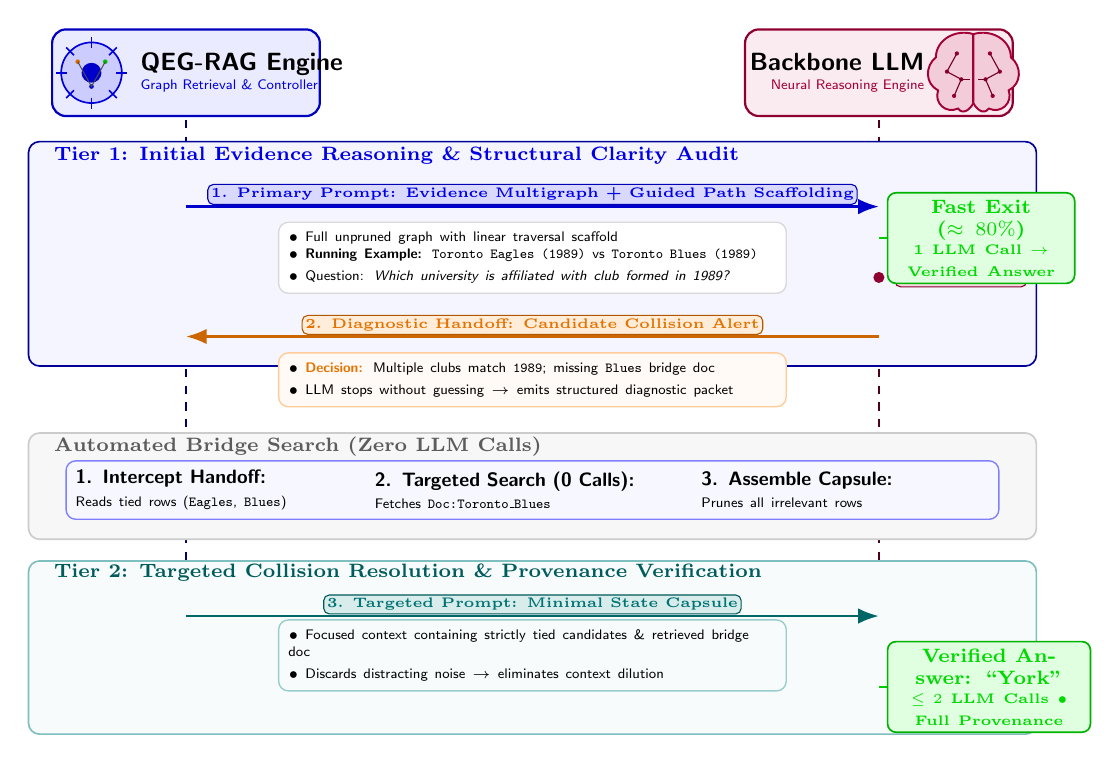
\begin{tikzpicture}[
  >=Latex,
  font=\sffamily\scriptsize,
  % Styles
  actor_box/.style={draw=#1!75!black, fill=#1!8, rounded corners=5pt, line width=0.8pt, inner sep=4pt},
  section_band/.style={draw=#1!60!black, fill=#1!4, rounded corners=4pt, line width=0.6pt},
  band_title/.style={font=\bfseries\scriptsize, text=#1!90!black, anchor=west},
  msg_card/.style={draw=gray!30, fill=white, rounded corners=3.5pt, line width=0.5pt, inner sep=3.5pt},
  badge/.style={fill=#1!15, draw=#1!70!black, line width=0.4pt, rounded corners=2pt, inner sep=1.2pt, font=\bfseries\tiny, text=#1!90!black},
  flow_arrow/.style={->, line width=1.0pt, draw=#1!80!black},
  exit_pill/.style={fill=green!12, draw=green!70!black, line width=0.6pt, rounded corners=3pt, inner sep=2.5pt, font=\bfseries\scriptsize, text=green!85!black, align=center}
]

% Define Brain Icon Macro
\def\drawbrain#1#2{
  \begin{scope}[shift={(#1)}, scale=#2]
    % Left hemisphere
    \draw[fill=purple!20, draw=purple!85!black, line width=0.7pt]
      (0, 0.7) 
      .. controls (-0.32, 0.8) and (-0.68, 0.6) .. (-0.68, 0.28)
      .. controls (-0.88, 0.12) and (-0.88, -0.2) .. (-0.64, -0.32)
      .. controls (-0.72, -0.55) and (-0.5, -0.75) .. (-0.28, -0.65)
      .. controls (-0.18, -0.78) and (-0.05, -0.65) .. (0, -0.55)
      -- cycle;
    % Right hemisphere
    \draw[fill=purple!20, draw=purple!85!black, line width=0.7pt]
      (0, 0.7) 
      .. controls (0.32, 0.8) and (0.68, 0.6) .. (0.68, 0.28)
      .. controls (0.88, 0.12) and (0.88, -0.2) .. (0.64, -0.32)
      .. controls (0.72, -0.55) and (0.5, -0.75) .. (0.28, -0.65)
      .. controls (0.18, -0.78) and (0.05, -0.65) .. (0, -0.55)
      -- cycle;
    % Central line
    \draw[purple!85!black, line width=0.7pt] (0, 0.68) -- (0, -0.53);
    % Neural nodes & synapses
    \fill[purple!80!black] (-0.3, 0.35) circle (1.1pt);
    \fill[purple!80!black] (-0.48, 0.02) circle (1.1pt);
    \fill[purple!80!black] (-0.22, -0.12) circle (1.1pt);
    \fill[purple!80!black] (-0.35, -0.42) circle (1.1pt);
    \draw[purple!60!black, line width=0.4pt] (-0.3, 0.35) -- (-0.48, 0.02) -- (-0.22, -0.12) -- (-0.35, -0.42);
    
    \fill[purple!80!black] (0.3, 0.35) circle (1.1pt);
    \fill[purple!80!black] (0.48, 0.02) circle (1.1pt);
    \fill[purple!80!black] (0.22, -0.12) circle (1.1pt);
    \fill[purple!80!black] (0.35, -0.42) circle (1.1pt);
    \draw[purple!60!black, line width=0.4pt] (0.3, 0.35) -- (0.48, 0.02) -- (0.22, -0.12) -- (0.35, -0.42);
    \draw[purple!60!black, line width=0.4pt, dashed] (-0.22, -0.12) -- (0.22, -0.12);
  \end{scope}
}

% Define Gear/System Icon Macro
\def\drawsystemicon#1#2{
  \begin{scope}[shift={(#1)}, scale=#2]
    \draw[fill=blue!20, draw=blue!85!black, line width=0.6pt] (0,0) circle (0.55);
    \fill[blue!80!black] (0,0) circle (0.18);
    \foreach \a in {0, 45, 90, 135, 180, 225, 270, 315} {
      \draw[blue!85!black, line width=0.6pt] (\a:0.45) -- (\a:0.65);
    }
    % Mini graph inside
    \fill[orange!85!black] (-0.25, 0.2) circle (1.2pt);
    \fill[green!75!black] (0.25, 0.2) circle (1.2pt);
    \fill[blue!85!black] (0, -0.25) circle (1.2pt);
    \draw[gray!60!black, line width=0.35pt] (-0.25, 0.2) -- (0, -0.25) -- (0.25, 0.2);
  \end{scope}
}

% Geometry:
% Width: 12.8cm, Left Actor X: 1.8cm, Right Actor X: 11.0cm
% Center X: 6.4cm

% ==========================================================
% TOP ACTOR HEADERS
% ==========================================================
% Actor 1: QEG-RAG Engine
\node[actor_box=blue, minimum width=3.4cm, minimum height=1.1cm] (act_qeg) at (2.0, 5.7) {};
\drawsystemicon{0.8, 5.7}{0.7};
\node[anchor=west, align=left] at (1.3, 5.7) {
  \textbf{\small QEG-RAG Engine}\\[-0.5mm]
  {\fontsize{5.2pt}{6.2pt}\selectfont \textcolor{blue!85!black}{Graph Retrieval \& Controller}}
};

% Actor 2: LLM Reasoner (Brain Icon)
\node[actor_box=purple, minimum width=3.4cm, minimum height=1.1cm] (act_llm) at (10.8, 5.7) {};
\drawbrain{12.0, 5.7}{0.7};
\node[anchor=east, align=right] at (11.5, 5.7) {
  \textbf{\small Backbone LLM}\\[-0.5mm]
  {\fontsize{5.2pt}{6.2pt}\selectfont \textcolor{purple!85!black}{Neural Reasoning Engine}}
};

% Vertical Actor Guidelines (Dotted)
\draw[blue!40!black, line width=0.6pt, dashed] (2.0, 5.1) -- (2.0, -2.5);
\draw[purple!40!black, line width=0.6pt, dashed] (10.8, 5.1) -- (10.8, -2.5);

% ==========================================================
% SECTION 1: TIER 1 INTERACTION
% ==========================================================
\node[section_band=blue, minimum width=12.8cm, minimum height=2.85cm] (sec_t1) at (6.4, 3.4) {};
\node[band_title=blue] at (0.2, 4.65) {\textbf{Tier 1: Initial Evidence Reasoning \& Structural Clarity Audit}};

% Step 1: Forward Message (QEG-RAG -> LLM)
\draw[flow_arrow=blue] (2.0, 4.0) -- (10.8, 4.0);
\node[badge=blue, anchor=south] at (6.4, 4.02) {1. Primary Prompt: Evidence Multigraph + Guided Path Scaffolding};

\node[msg_card, text width=6.2cm, align=left] at (6.4, 3.35) {
  {\fontsize{5.2pt}{6.2pt}\selectfont
  $\bullet$ Full unpruned graph with linear traversal scaffold\\
  $\bullet$ \textbf{Running Example:} \texttt{Toronto Eagles (1989)} vs \texttt{Toronto Blues (1989)}\\
  $\bullet$ Question: \textit{Which university is affiliated with club formed in 1989?}}
};

% Evaluation in LLM
\fill[purple!75!black] (10.8, 3.1) circle (2pt);
\node[badge=purple, anchor=west] at (11.0, 3.1) {Clarity Audit};

% Fast Exit Branch (Right)
\draw[flow_arrow=green] (10.8, 3.6) -- (12.5, 3.6);
\node[exit_pill, text width=2.2cm, anchor=west] at (10.9, 3.6) {
  \textbf{Fast Exit ($\approx 80\%$)}\\[-0.4mm]
  {\fontsize{4.8pt}{5.5pt}\selectfont 1 LLM Call $\to$ Verified Answer}
};

% Collision Return Arrow (LLM -> QEG-RAG)
\draw[flow_arrow=orange] (10.8, 2.35) -- (2.0, 2.35);
\node[badge=orange, anchor=south] at (6.4, 2.37) {2. Diagnostic Handoff: Candidate Collision Alert};

\node[msg_card, draw=orange!40, fill=orange!4, text width=6.2cm, align=left] at (6.4, 1.8) {
  {\fontsize{5.2pt}{6.2pt}\selectfont
  $\bullet$ \textcolor{orange!90!black}{\textbf{Decision:}} Multiple clubs match \texttt{1989}; missing \texttt{Blues} bridge doc\\
  $\bullet$ LLM stops without guessing $\to$ emits structured diagnostic packet}
};

% ==========================================================
% SECTION 2: ZERO-LLM TARGETED BRIDGE RETRIEVAL
% ==========================================================
\node[section_band=gray, fill=gray!6, draw=gray!40, minimum width=12.8cm, minimum height=1.35cm] (sec_bridge) at (6.4, 0.45) {};
\node[band_title=gray!80!black] at (0.2, 0.95) {\textbf{Automated Bridge Search (Zero LLM Calls)}};

% Processing inside QEG-RAG
\node[msg_card, draw=blue!50, fill=blue!3, text width=11.6cm, align=left] at (6.4, 0.4) {
  \begin{minipage}{0.32\linewidth}
    \textbf{1. Intercept Handoff:}\\
    {\fontsize{5.0pt}{5.8pt}\selectfont Reads tied rows (\texttt{Eagles}, \texttt{Blues})}
  \end{minipage}
  \begin{minipage}{0.35\linewidth}
    \textbf{2. Targeted Search (0 Calls):}\\
    {\fontsize{5.0pt}{5.8pt}\selectfont Fetches \texttt{Doc:Toronto\_Blues}}
  \end{minipage}
  \begin{minipage}{0.30\linewidth}
    \textbf{3. Assemble Capsule:}\\
    {\fontsize{5.0pt}{5.8pt}\selectfont Prunes all irrelevant rows}
  \end{minipage}
};

% ==========================================================
% SECTION 3: TIER 2 INTERACTION
% ==========================================================
\node[section_band=teal, fill=teal!3, draw=teal!50, minimum width=12.8cm, minimum height=2.2cm] (sec_t2) at (6.4, -1.6) {};
\node[band_title=teal!80!black] at (0.2, -0.65) {\textbf{Tier 2: Targeted Collision Resolution \& Provenance Verification}};

% Step 3: Forward Message (QEG-RAG -> LLM)
\draw[flow_arrow=teal] (2.0, -1.2) -- (10.8, -1.2);
\node[badge=teal, anchor=south] at (6.4, -1.18) {3. Targeted Prompt: Minimal State Capsule};

\node[msg_card, draw=teal!40, fill=teal!3, text width=6.2cm, align=left] at (6.4, -1.7) {
  {\fontsize{5.2pt}{6.2pt}\selectfont
  $\bullet$ Focused context containing strictly tied candidates \& retrieved bridge doc\\
  $\bullet$ Discards distracting noise $\to$ eliminates context dilution}
};

% Final Verified Resolution Arrow from LLM
\draw[flow_arrow=green] (10.8, -2.1) -- (12.5, -2.1);
\node[exit_pill, text width=2.4cm, anchor=west] at (10.9, -2.1) {
  \textbf{Verified Answer: ``York''}\\[-0.4mm]
  {\fontsize{4.8pt}{5.5pt}\selectfont $\le 2$ LLM Calls $\bullet$ Full Provenance}
};

\end{tikzpicture}
\end{document}
